\documentclass[12pt,letterpaper]{article}
\usepackage{anysize}
\usepackage{amsmath}
\marginsize{2cm}{2cm}{1cm}{1cm}
\usepackage{listings}
\usepackage{cite}
\usepackage{caption}
\usepackage{upquote}
\usepackage{xcolor}
\usepackage{xcolor}

\usepackage{tikz}
\def\checkmark{\tikz\fill[scale=0.4](0,.35) -- (.25,0) -- (1,.7) -- (.25,.15) -- cycle;} 

\usepackage{graphicx}


\begin{document}

\begin{titlepage}
    \vspace*{4cm}
    \begin{flushleft}
    {\huge
        CS519 Project 4\\[.5cm]
    }
    {\large
        Interactive Noisy Elliptical Polka-dots
    }
    \end{flushleft}
    \vfill
    \rule{5in}{.5mm}\\
    Li Li

\end{titlepage}
\section{source files}
There are only three files ovalnoise.frag, ovalnoise.glib and ovalnoise.vert.
\section{a simple explanation}
What I did are:\\
\begin{tabular}{ |l | c |}
  \hline                       
  \bf{Feature} & \bf{Status} \\ \hline
  uAd and uBd & \checkmark \\ \hline
  uNoiseAmp & \checkmark \\ \hline
  uNoiseFreq & \checkmark \\ \hline
  uTol & \checkmark \\ \hline
  uAlpha & \checkmark \\ \hline
  ChromaDepth & \checkmark \\ \hline
\end{tabular}

\begin{itemize}
\item For uAd and uBd, it just looks like previous ellipse parameter claim in glib file pass to vert file. It similar create numinu and numinv with these two parameter. And with them I do calculate dis from centre to edge of an ellipse. Which is ((up - uc)*2./uAd)*((up - uc)*2./uAd) + ((vp - vc)*2./uBd)*((vp - vc)*2./uBd). Now I since orange to those in ellipse. See Figure 1.
\item Now for the noise, I go to NoiseWithGlman.pdf. And it can work very simple add this pre-created uniform variable called Noise3. uNoiseFreq is a parameter to texture3D fuction whether uNoiseAmp need to simply times the noise value. After these adding this noise value to up. One is enough, not need to add to vp. See Figure 2.
\item Now I come to most tricky one in the project I think, I don't understand in the beginning. But later I figure out With this uTol, my distance of centre to edge of an ellipse changed a little bit. Originally, distance is 1.0 from centre to edge. Now it can be 1.0+uTol. And for pixel located in 1.0-uTol to 1.0+uTol we sign them color base on distance to centre. These color is mixed by orange and white. The smoothstep function is exactly doing this. See Figure 3.
\item uAlpha, I add it after sign uTol color. It only changed alpha value of gl\_FragColor. Not very hard. See Figure 4. This vase is two layered, so it does not show a simple transparent object.
\item Finally, for ChromaDepth, I just follow the instruction. Set parameters, use the rainbow function. Set Z depth value from eye coordinate. Just figure out need to blend the color comes out from rainbow function. And I set a uBlend parameter. It seems that with bigger positive uBlend the result seems better. See Fugure 5. 
\end{itemize}
\section{result}

\begin{figure}[p]
    \centering
    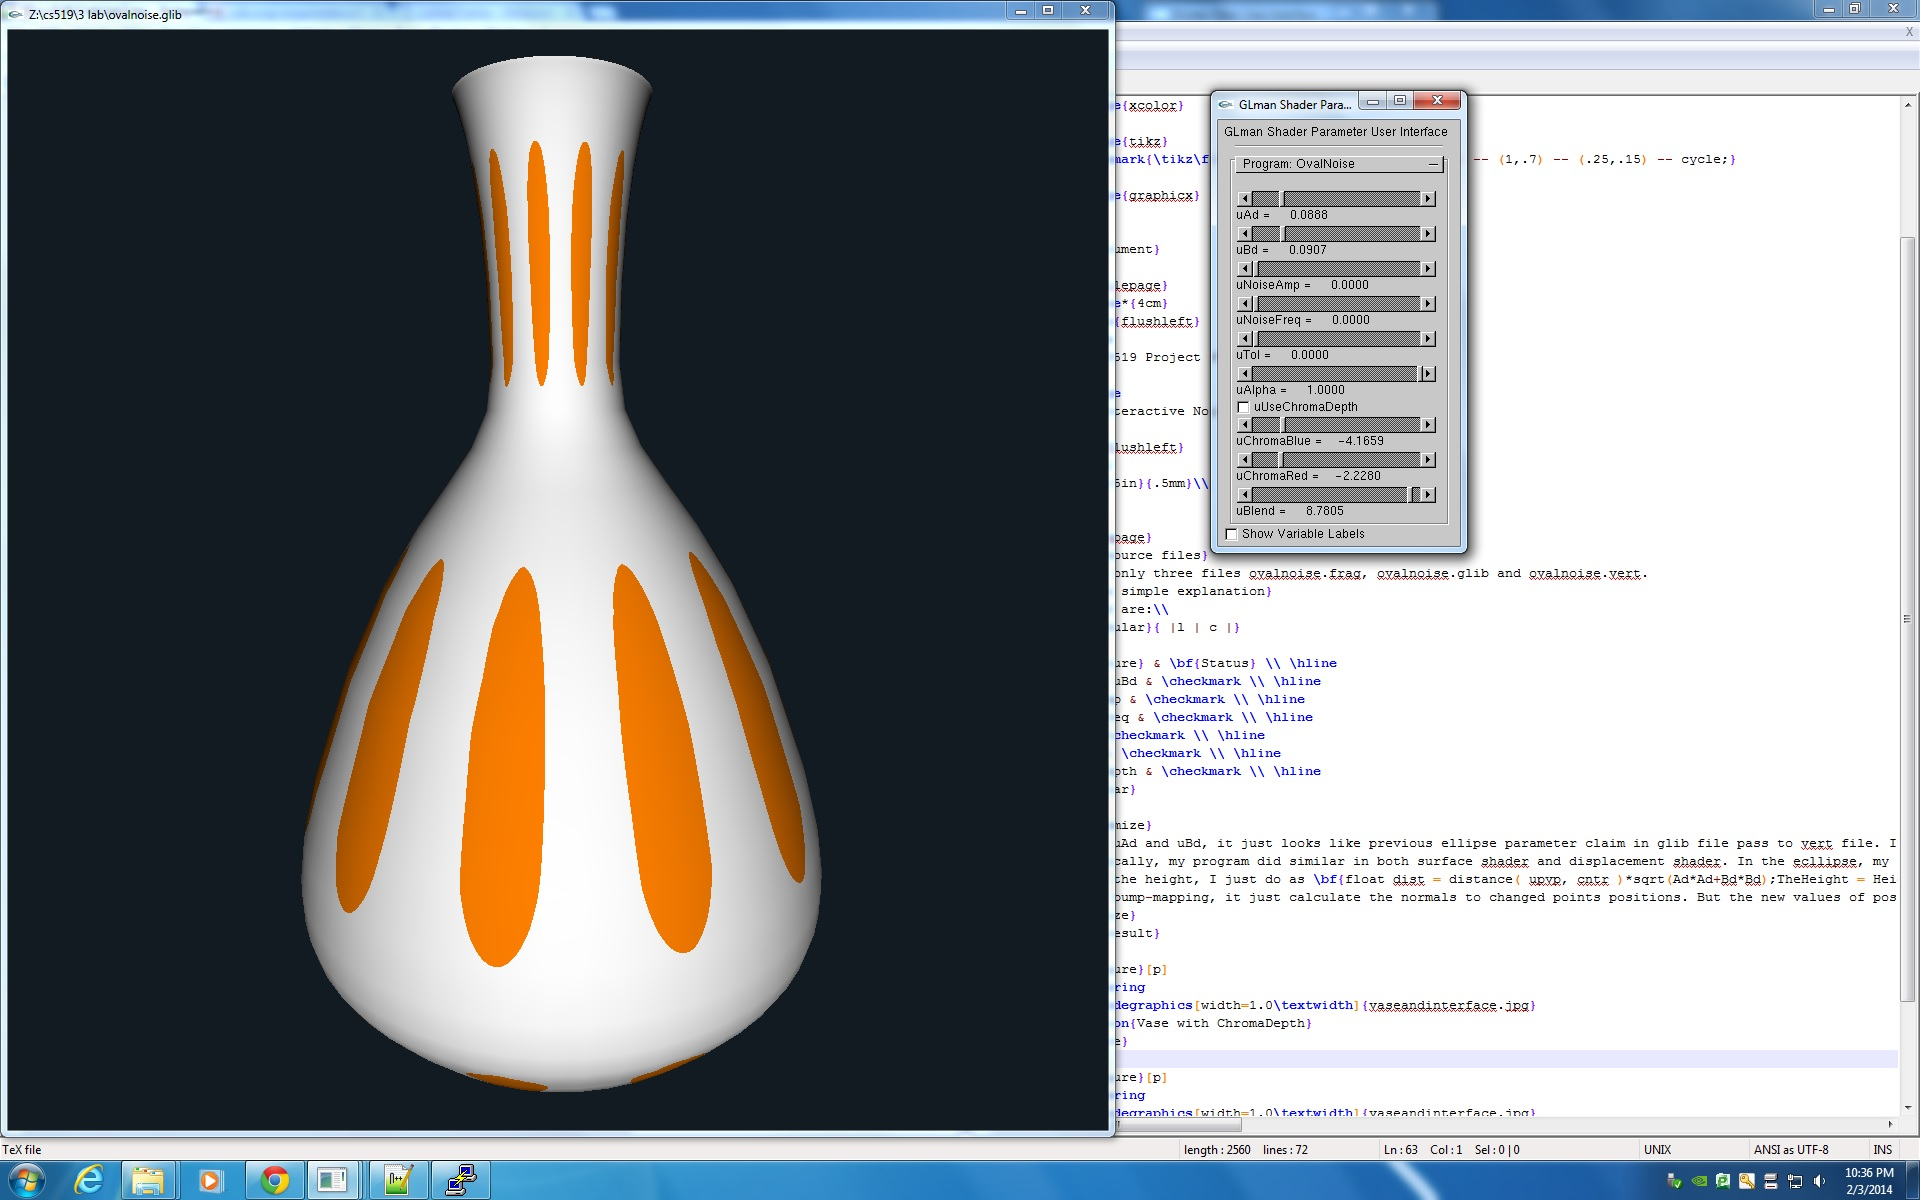
\includegraphics[width=1.0\textwidth]{ellipse.jpg}
    \caption{Vase with ellipses}
\end{figure}

\begin{figure}[p]
    \centering
    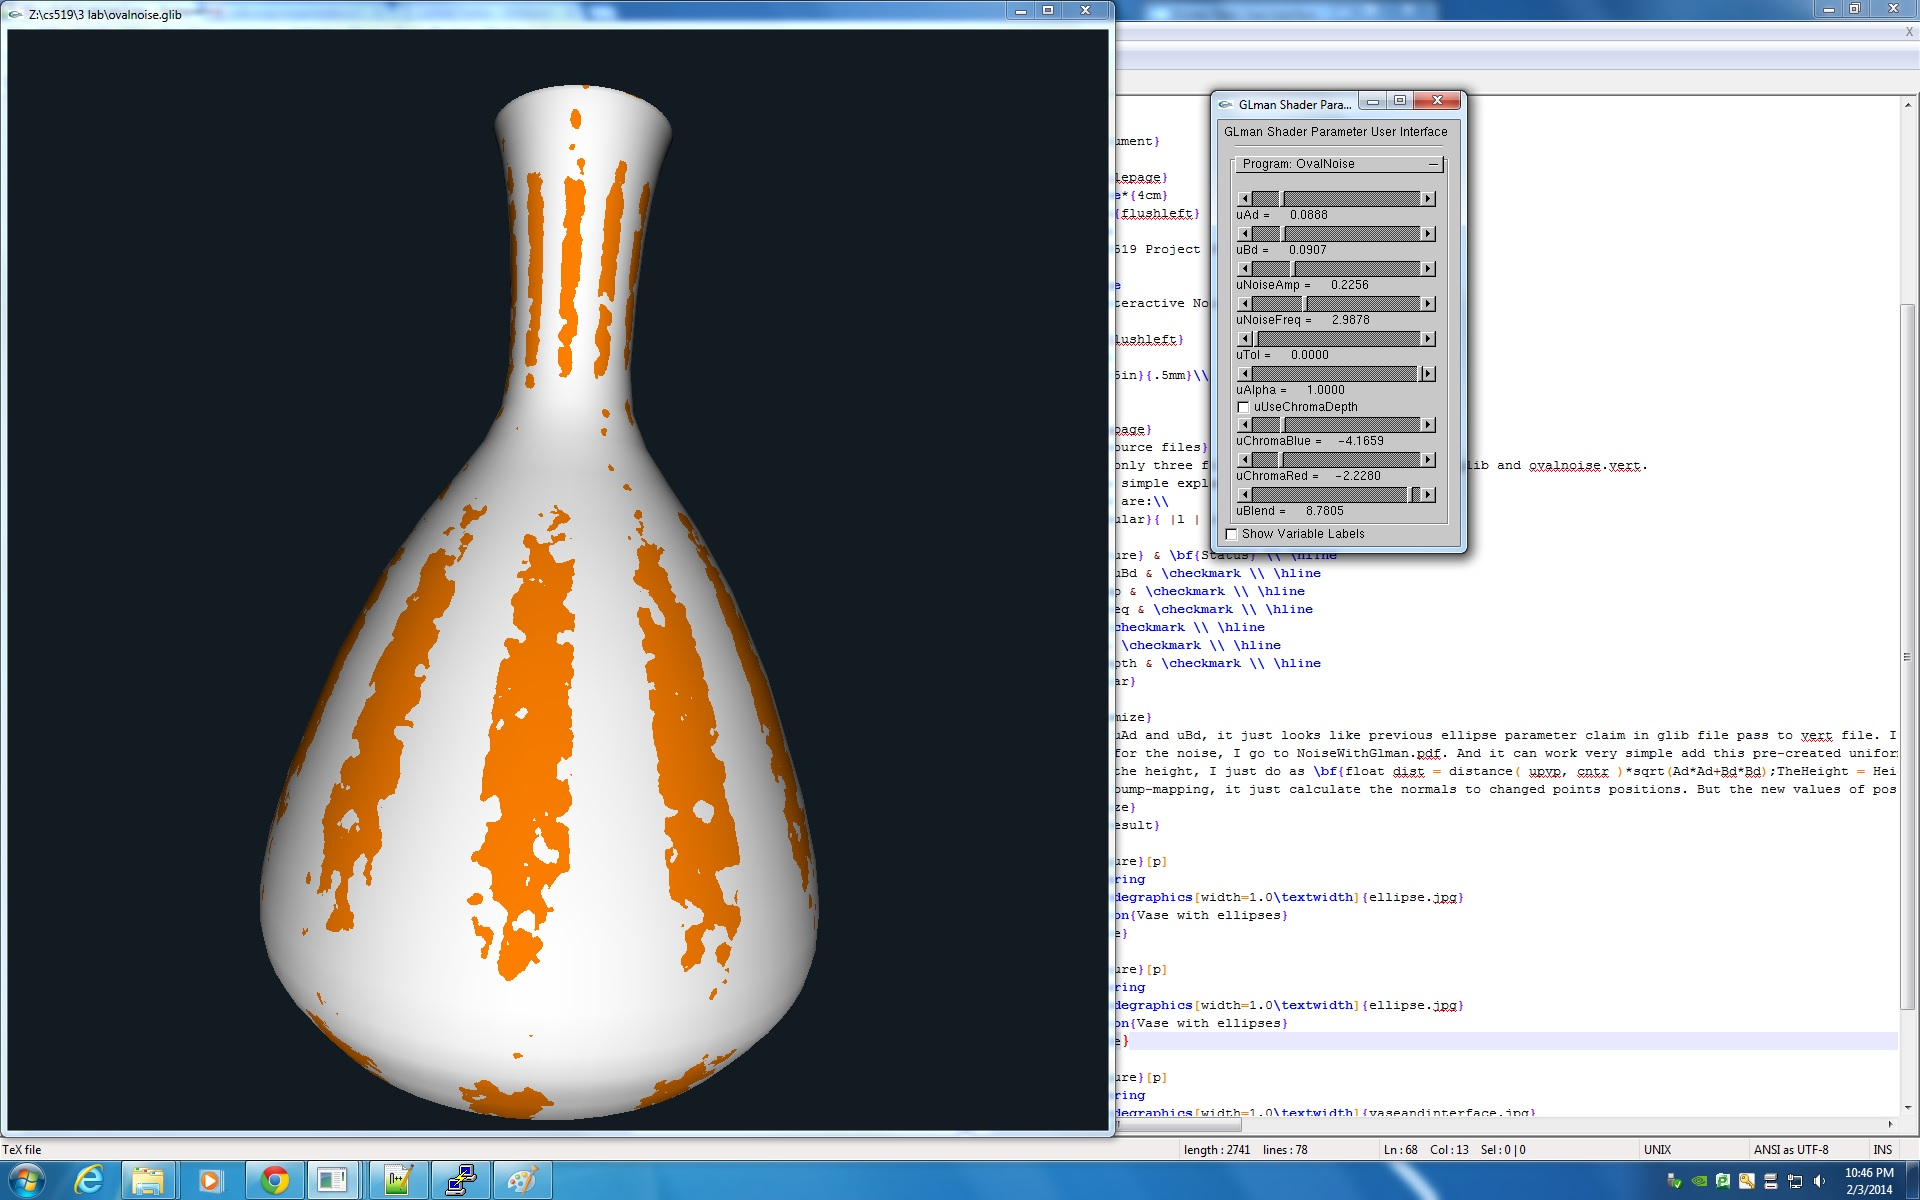
\includegraphics[width=1.0\textwidth]{noise.jpg}
    \caption{Vase with noise}
\end{figure}

\begin{figure}[p]
    \centering
    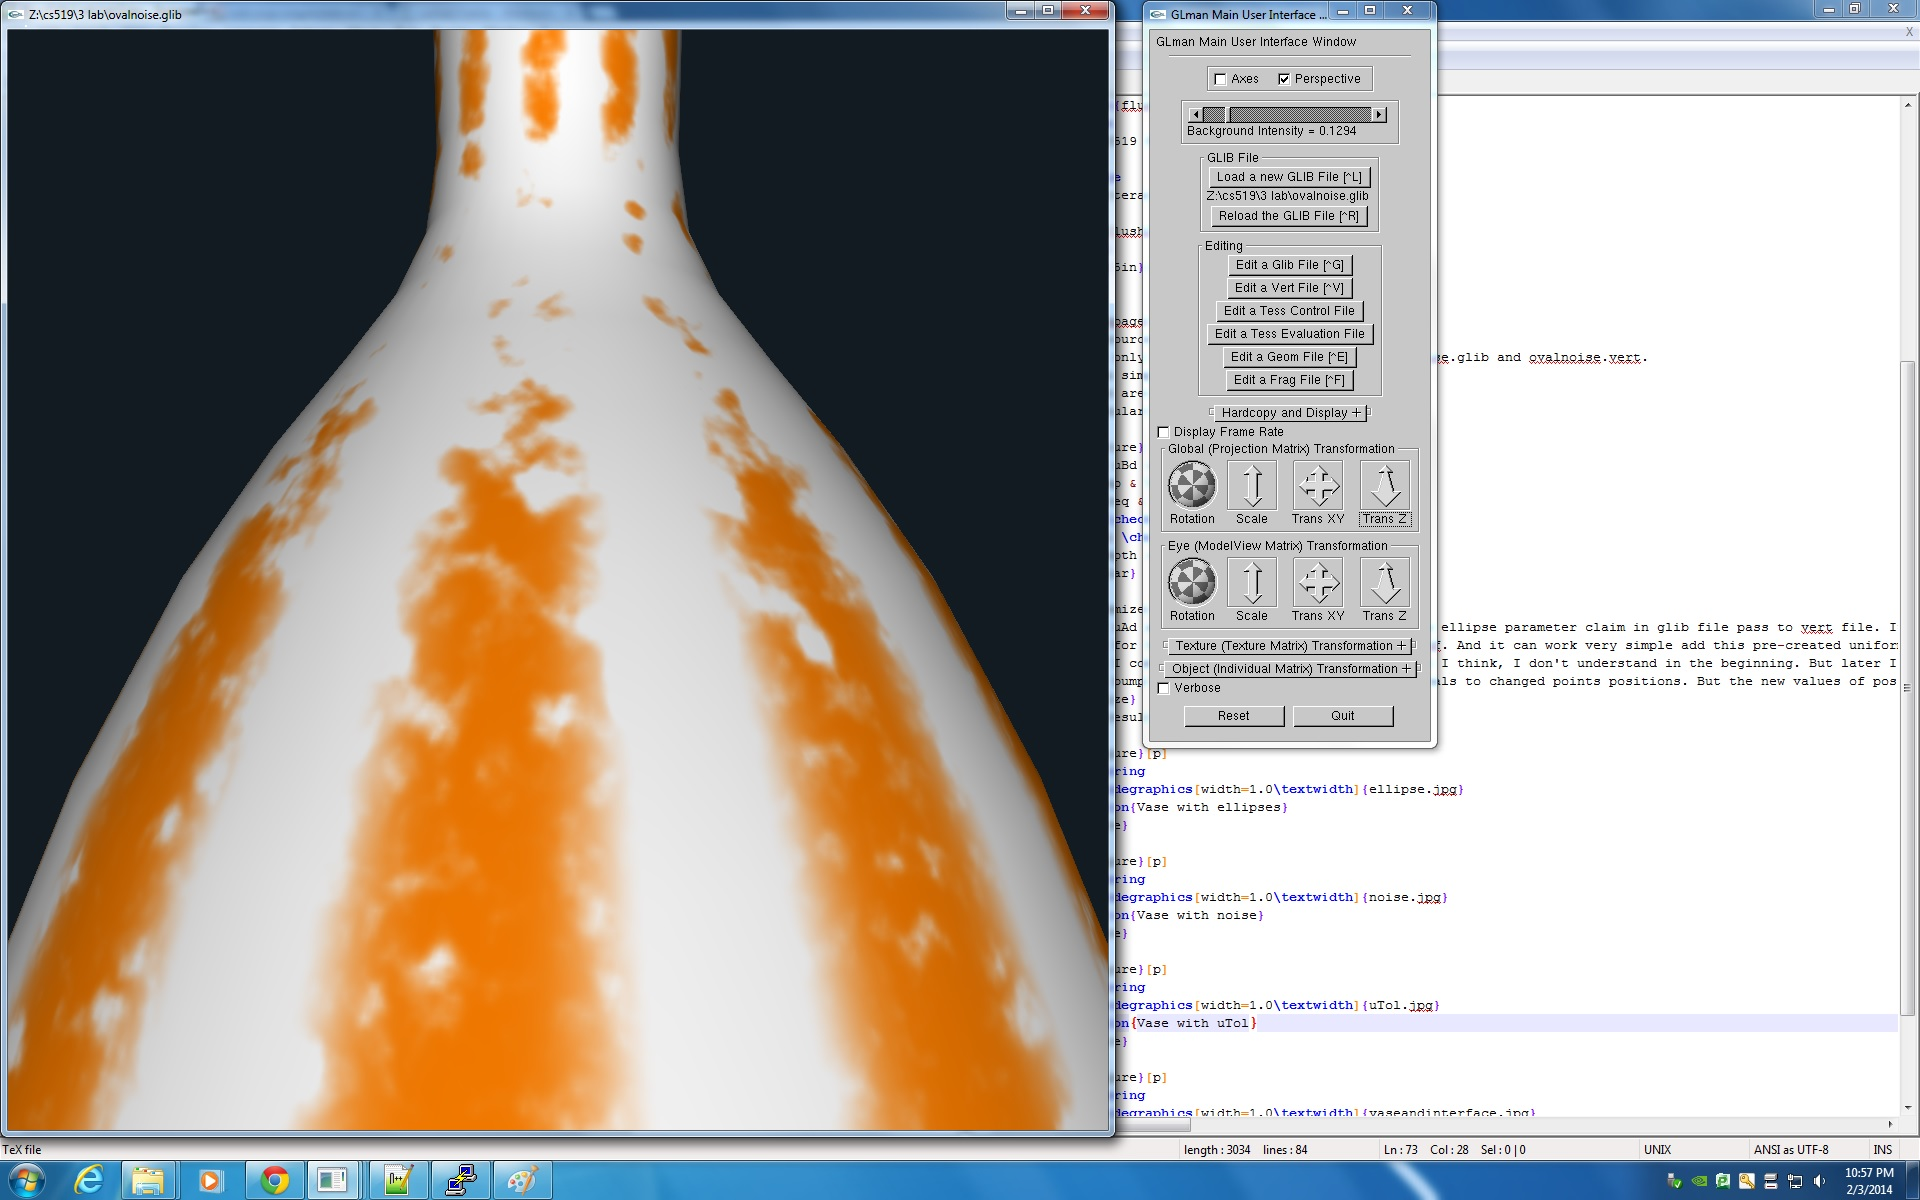
\includegraphics[width=1.0\textwidth]{uTol.jpg}
    \caption{Vase with uTol}
\end{figure}

\begin{figure}[p]
    \centering
    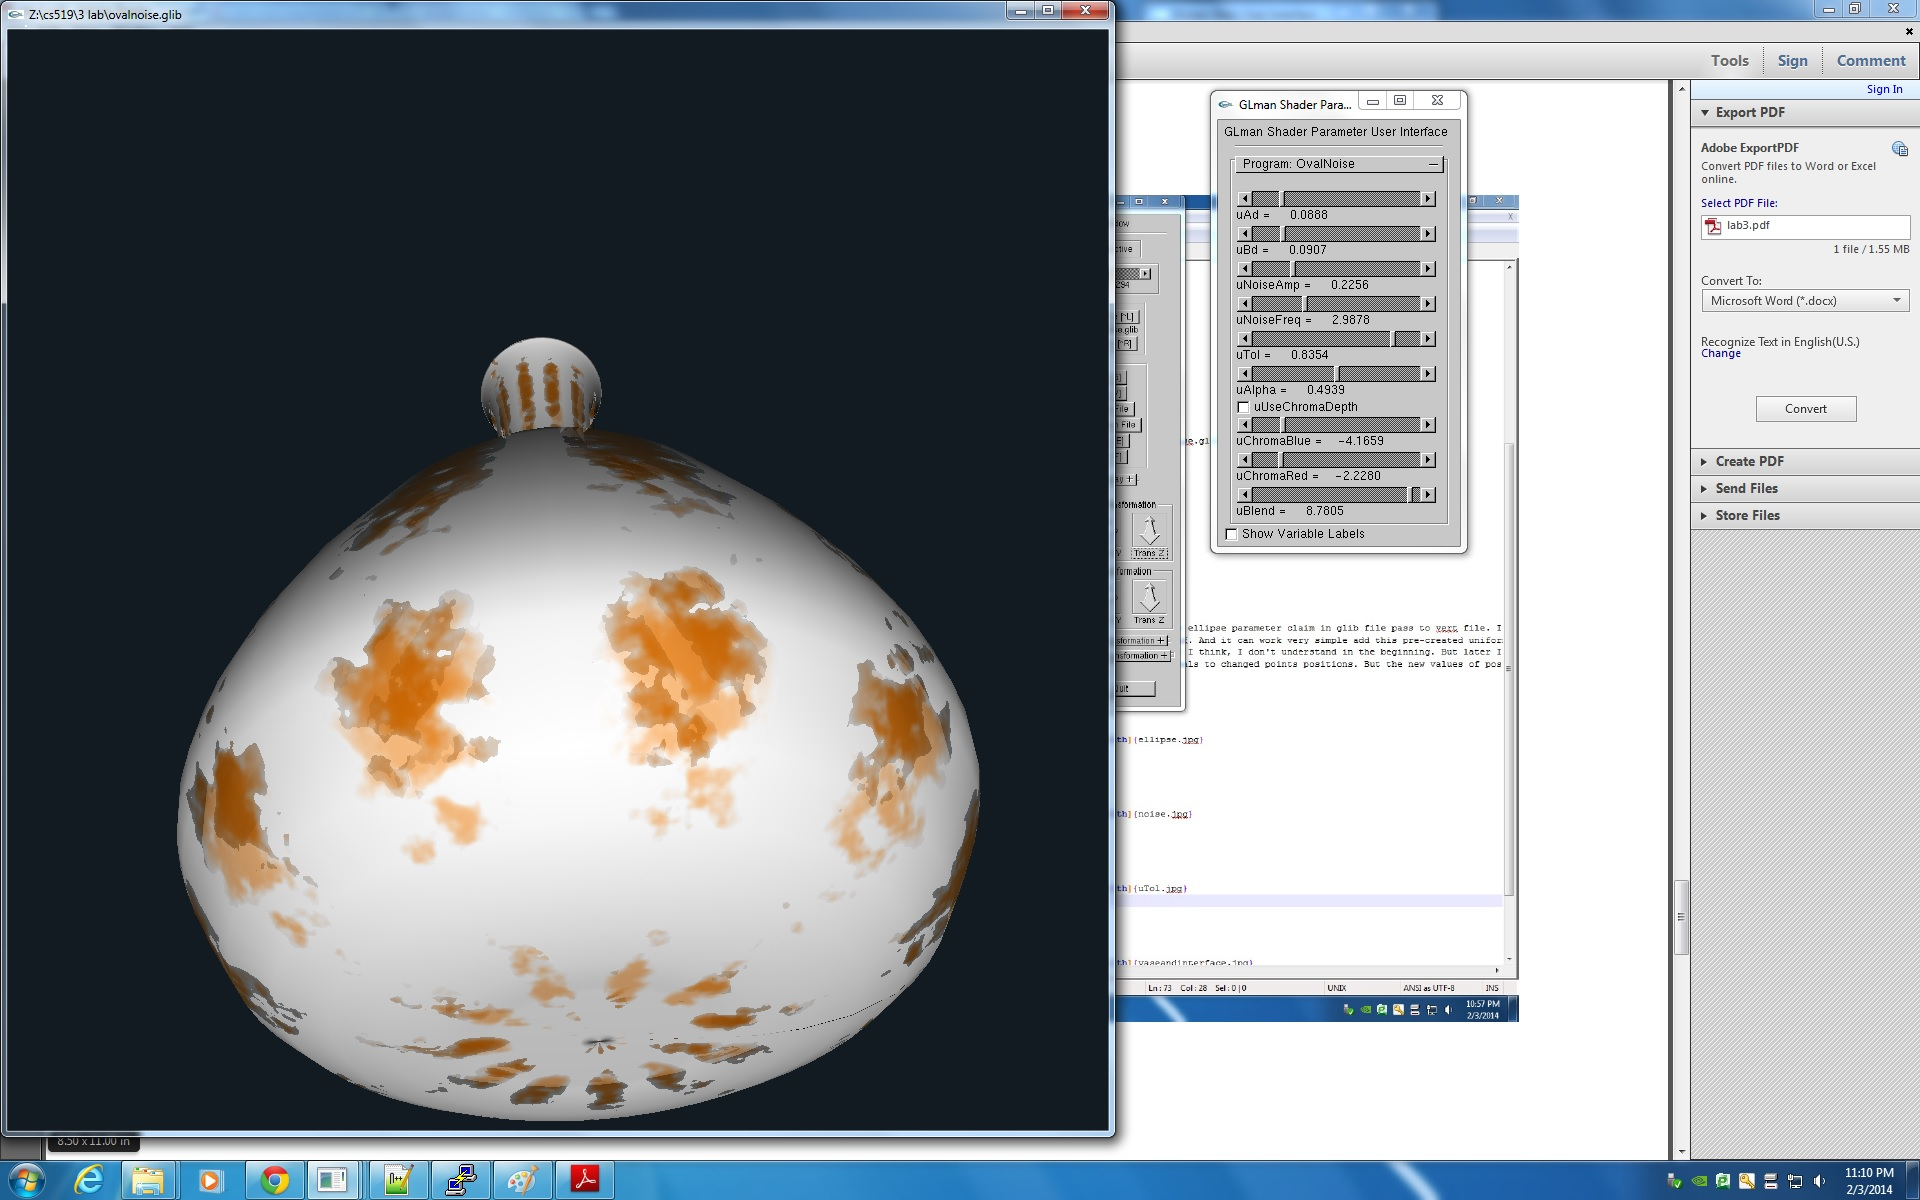
\includegraphics[width=1.0\textwidth]{Alpha.jpg}
    \caption{Vase with Alpha}
\end{figure}

\begin{figure}[p]
    \centering
    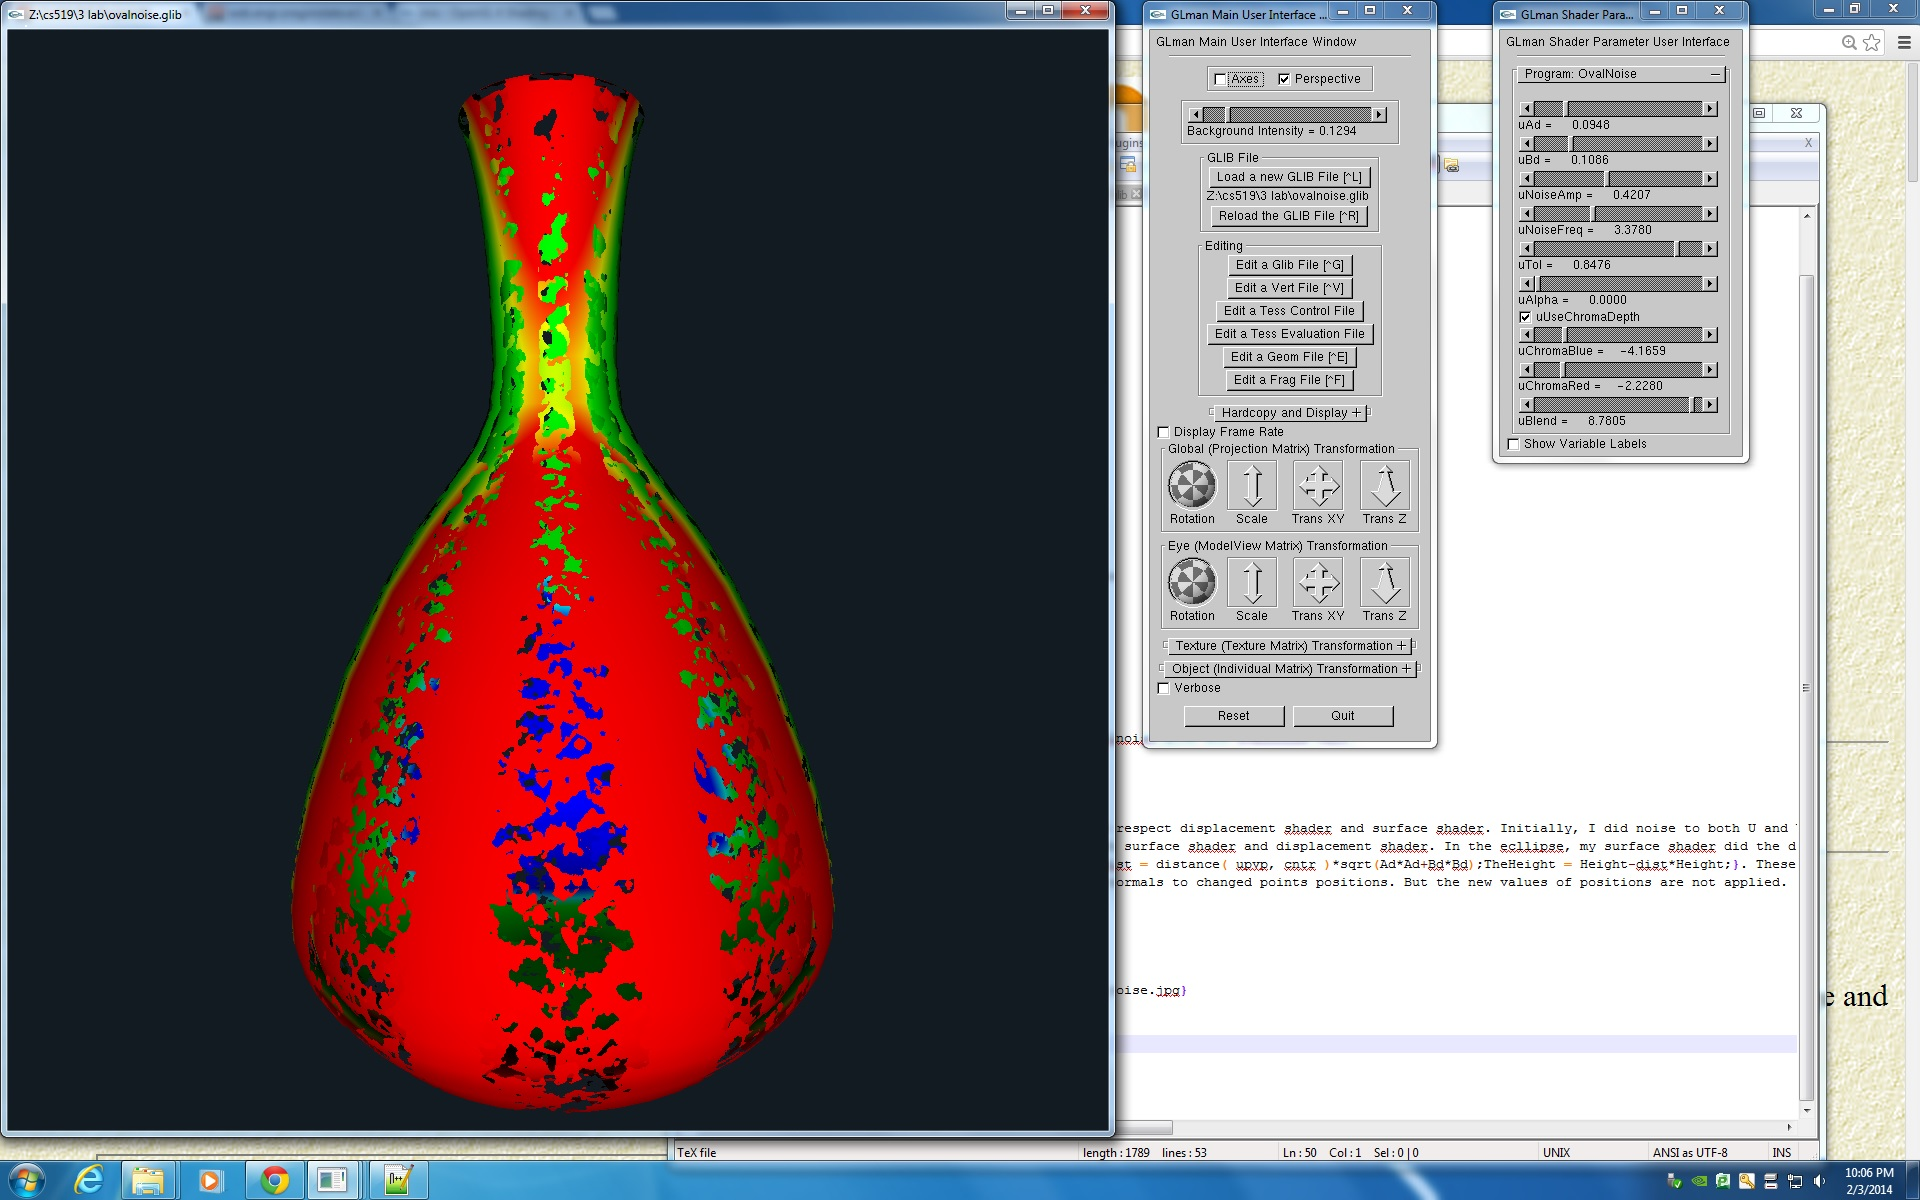
\includegraphics[width=1.0\textwidth]{vaseandinterface.jpg}
    \caption{Vase with ChromaDepth}
\end{figure}


\end {document}
